% LaTeX snippets for figures. Embed inline in main.tex near relevant text.

\begin{figure}[t]
  \centering
  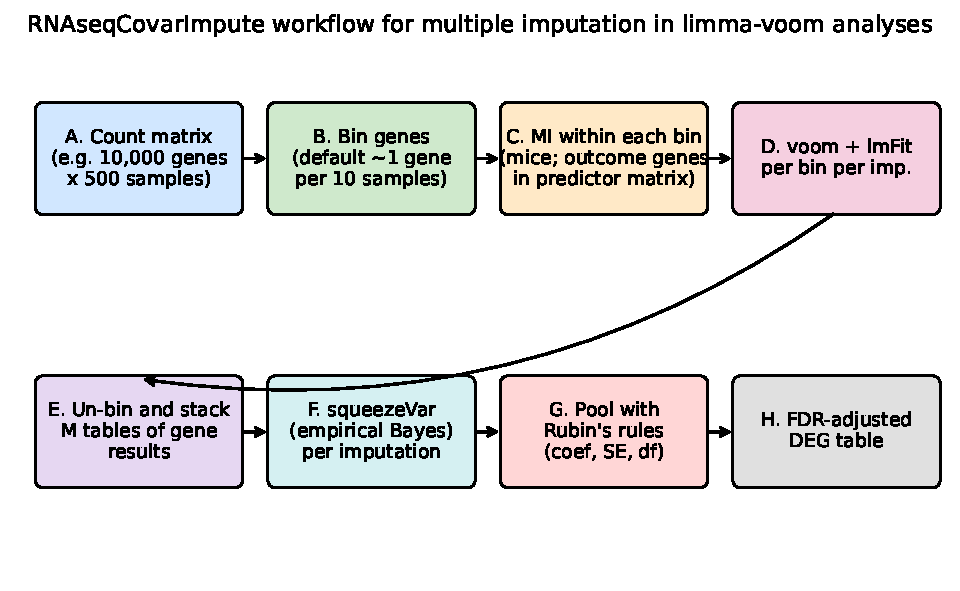
\includegraphics[width=0.95\linewidth]{figures/fig1.pdf}
  \caption{Overview of the RNAseqCovarImpute workflow. (A) The raw count matrix
  (example: 10,000 genes $\times$ 500 samples) is (B) partitioned into small
  gene bins (default: approximately one gene per ten samples), (C) $M$ imputed
  datasets are constructed independently within each bin using mice, with the
  log-CPM values of the bin's genes included in the imputation predictor
  matrix, and (D) limma-voom with a globally fit mean-variance trend is applied
  per bin per imputation. (E) Gene-level results are un-binned and stacked
  across imputations, (F) squeezeVar empirical-Bayes variance shrinkage is
  applied per imputation, and (G) Rubin's rules pool coefficients, standard
  errors, and Barnard--Rubin adjusted degrees of freedom. (H) The pooled
  P-values are FDR-adjusted.}
  \label{fig:method}
\end{figure}

\begin{figure}[t]
  \centering
  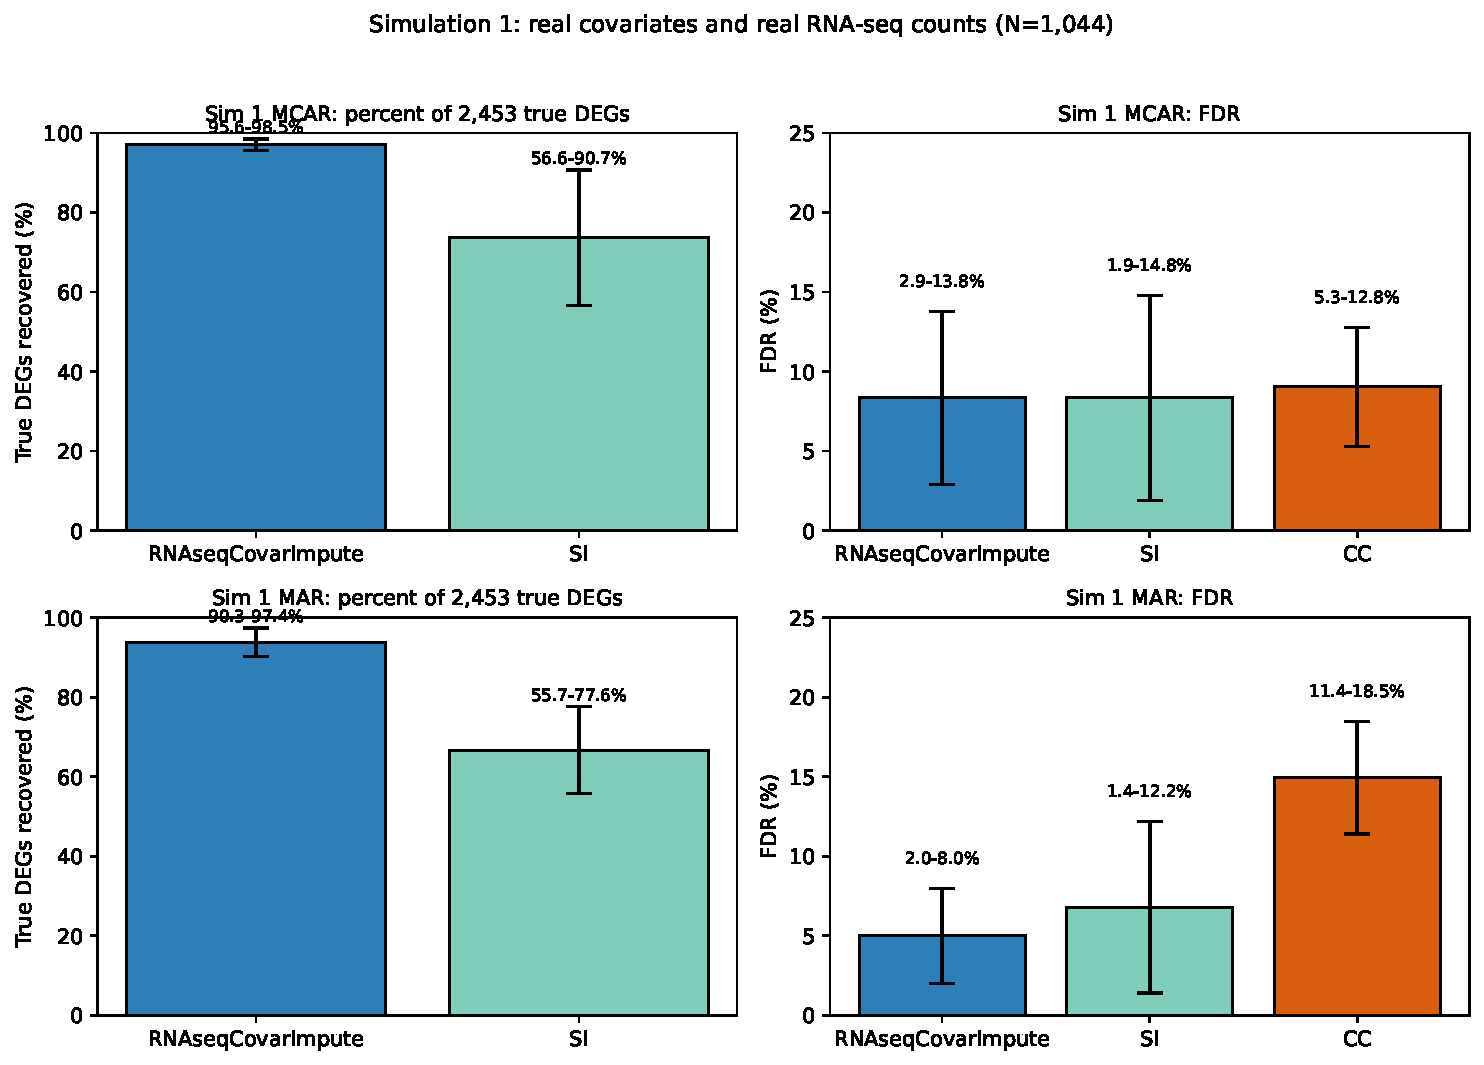
\includegraphics[width=0.95\linewidth]{figures/fig2.pdf}
  \caption{Simulation 1: real ECHO-PATHWAYS placental covariates and real
  RNA-seq counts ($N=1{,}044$; 2{,}453 full-data true DEGs). Bars show the
  observed range of each metric across missingness levels from 5\% to 55\%
  under MCAR (top) and MAR (bottom) mechanisms. RNAseqCovarImpute recovers
  95.6--98.5\% of true DEGs under MCAR and 90.3--97.4\% under MAR, compared
  with 56.6--90.7\% and 55.7--77.6\% for single imputation. FDR is comparable
  across methods under MCAR (MI 2.9--13.8\%, SI 1.9--14.8\%, CC 5.3--12.8\%)
  but rises for complete case under MAR (CC 11.4--18.5\%).}
  \label{fig:sim1}
\end{figure}

\begin{figure}[t]
  \centering
  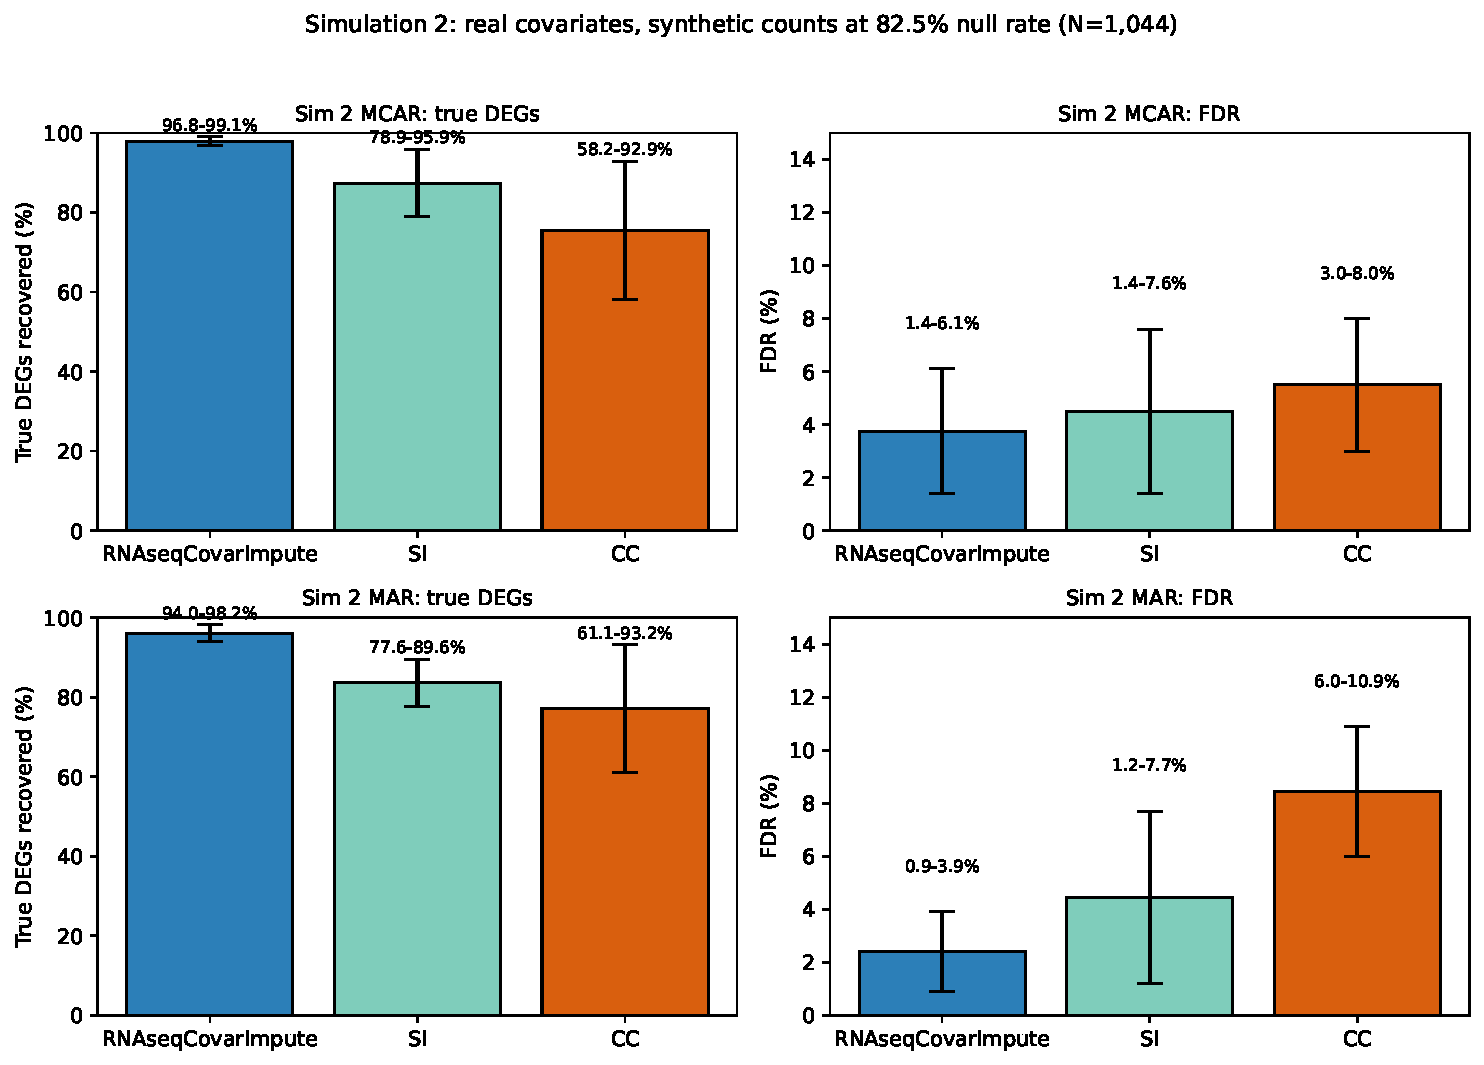
\includegraphics[width=0.95\linewidth]{figures/fig3.pdf}
  \caption{Simulation 2: real covariates combined with seqgendiff synthetic
  counts at an 82.5\% null-gene rate ($N=1{,}044$). Under MCAR,
  RNAseqCovarImpute recovers 96.8--99.1\% of true DEGs versus 78.9--95.9\%
  for SI and 58.2--92.9\% for CC, with comparable FDR (MI 1.4--6.1\%,
  SI 1.4--7.6\%) and higher CC FDR (3.0--8.0\%). MAR patterns mirror MCAR,
  with true-DEG recovery 94.0--98.2\% (MI), 77.6--89.6\% (SI), 61.1--93.2\%
  (CC) and FDR 0.9--3.9\%, 1.2--7.7\%, 6.0--10.9\% respectively.}
  \label{fig:sim2}
\end{figure}

\begin{figure}[t]
  \centering
  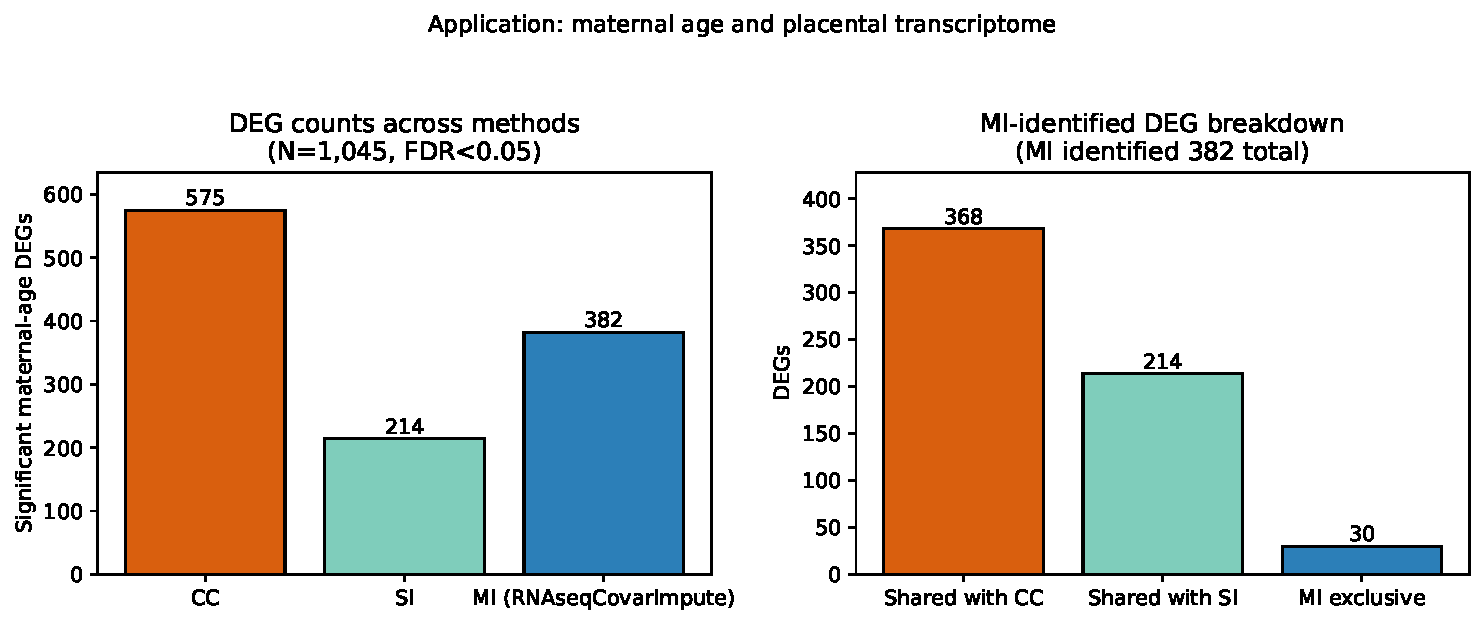
\includegraphics[width=0.95\linewidth]{figures/fig4.pdf}
  \caption{Application to maternal age and the placental transcriptome
  ($N=1{,}045$; 6\% of individuals missing at least one of ten covariates).
  The complete case, single imputation, and multiple imputation analyses
  identify 575, 214, and 382 differentially expressed genes respectively
  (left). Of the 382 MI-identified DEGs, CC captures 368 (96\%) and SI
  captures 214 (56\%); 30 DEGs are MI-exclusive (right).}
  \label{fig:app}
\end{figure}
